%%%%%%%%%%%%%%%%%%%%%%%%%%%%%%%%%%%%%%%%%
% Presentación de avance — Generative Deep Learning
% Detección generativa de degradación de suelo en monocultivos de pino
% Estilo: tema Boadilla con colores UdeC
%%%%%%%%%%%%%%%%%%%%%%%%%%%%%%%%%%%%%%%%%

\documentclass[10pt,aspectratio=169]{beamer}

\usetheme{Boadilla}

\usepackage[utf8]{inputenc}
\usepackage[spanish]{babel}
\usepackage{amsmath, amssymb, amsfonts}
\usepackage{graphicx}
\usepackage{xcolor}
\usepackage{booktabs}

\graphicspath{{figuras/}}

\definecolor{UdeCRed}{HTML}{9D2235}
\definecolor{UdeCGray}{HTML}{58585A}
\definecolor{UdeCLightGray}{HTML}{F0F0F0}

\setbeamercolor{palette primary}{use=structure,fg=white,bg=UdeCRed}
\setbeamercolor{palette secondary}{use=structure,fg=white,bg=UdeCGray}
\setbeamercolor{palette tertiary}{use=structure,fg=white,bg=UdeCGray}
\setbeamercolor{palette quaternary}{fg=black,bg=UdeCLightGray}

\setbeamercolor{title}{fg=UdeCRed,bg=white}
\setbeamercolor{frametitle}{fg=white,bg=UdeCRed}
\setbeamercolor{structure}{fg=UdeCRed}
\setbeamercolor{block title}{use=palette secondary,fg=white,bg=UdeCGray}
\setbeamercolor{block body}{use=palette quaternary,fg=black,bg=UdeCLightGray}

\definecolor{UdeCRedLight}{HTML}{E5A6B0}

\setbeamertemplate{footline}
{%
  \leavevmode%
  \hbox{%
  \begin{beamercolorbox}[wd=.85\paperwidth,ht=2.25ex,dp=1ex,left]{section in head/foot}%
    \insertsectionnavigationhorizontal{.85\paperwidth}{\hskip0pt plus1fill}{\hskip0pt plus1fill}
  \end{beamercolorbox}%
  \begin{beamercolorbox}[wd=.15\paperwidth,ht=2.25ex,dp=1ex,right]{author in head/foot}%
    \usebeamerfont{author in head/foot}\insertshortauthor\hspace*{2ex}
  \end{beamercolorbox}}%
  \vskip0pt%
}

\setbeamercolor{author in head/foot}{bg=white, fg=black}
\setbeamercolor{section in head/foot}{bg=UdeCRed, fg=white}
\setbeamercolor{section in head/foot shaded}{bg=UdeCRedLight, fg=white}

\title[Avance VAE]{Detección generativa de degradación de suelo\\en monocultivos de pino}
\subtitle{Presentación de avance --- Generative Deep Learning}
\author[M. Salgado]{Mario César Salgado Orellana}
\institute[UdeC]{Universidad de Concepción}
\date{9 de octubre de 2026}

\begin{document}

{
  \setbeamercolor{background canvas}{bg=white}
  \begin{frame}[plain]
    \titlepage
  \end{frame}
}

\begin{frame}
  \frametitle{Contenido}
  \tableofcontents
\end{frame}

% --- SECCIÓN 1 ---
\section[Problema]{Problema y propuesta}

\begin{frame}
  \frametitle{Problema y propuesta}
  \small
  \begin{columns}[T]
    \begin{column}{.48\textwidth}
      \begin{block}{Problema}
        \begin{itemize}\itemsep0.3em
          \item En la temporada 2022--2023 se quemaron \textbf{431.657 hectáreas} en Chile.
          \item La tala rasa también deja el suelo desnudo: una cuenca recién talada puede perder unas \textbf{87 veces más suelo} que una sin intervenir.
          \item Hoy se vigila el incendio mientras ocurre, pero casi no se hace seguimiento del terreno \textbf{después} del daño.
        \end{itemize}
      \end{block}
    \end{column}
    \begin{column}{.48\textwidth}
      \begin{block}{Propuesta}
        \begin{enumerate}\itemsep0.3em
          \item Descargar imágenes satelitales Sentinel-2 desde Google Earth Engine.
          \item Cortarlas en cuadrados (parches) de 640 m con 4 capas de información.
          \item Entrenar un VAE \textbf{solo con terreno sano}, para que aprenda cómo se ve lo normal.
          \item Si el modelo reconstruye mal un parche, es porque no se parece a lo sano: ese error es el \textbf{puntaje de daño}.
        \end{enumerate}
      \end{block}
    \end{column}
  \end{columns}
  \vspace{0.6em}
  \textbf{¿Para quién?} Al sector público le sirve para decidir dónde restaurar con especies nativas; al privado, para vigilar sus predios.

  \vfill
  {\tiny Fuentes: Gobierno de Chile / CONAF, balance 2022--2023; Revista Bosque (2024).}
\end{frame}

% --- SECCIÓN 2 ---
\section[Dataset]{Dataset y preprocesamiento}

\begin{frame}
  \frametitle{Fuente de datos y zona piloto}
  \small
  \begin{columns}[c]
    \begin{column}{.55\textwidth}
      \begin{itemize}\itemsep0.35em
        \item \textbf{Satélite:} Sentinel-2 nivel 2A. Son imágenes ya corregidas por la atmósfera, con píxeles de 10 $\times$ 10 m.
        \item \textbf{Herramienta:} Google Earth Engine, una plataforma de Google para descargar y procesar imágenes satelitales.
        \item \textbf{Zona piloto:} unos 71 $\times$ 89 km en Biobío, afectada por los incendios de 2023. En el mapa se ve el río Biobío y, en verde claro, la cicatriz del incendio.
        \item \textbf{Resultado:} una sola imagen de toda la zona, que Earth Engine cortó en \textbf{6 archivos} (3 filas $\times$ 2 columnas) porque era muy grande.
        \item Los bordes se ven un poco inclinados por la proyección (UTM, en metros). Las esquinas vacías no se usan.
      \end{itemize}
    \end{column}
    \begin{column}{.42\textwidth}
      \centering
      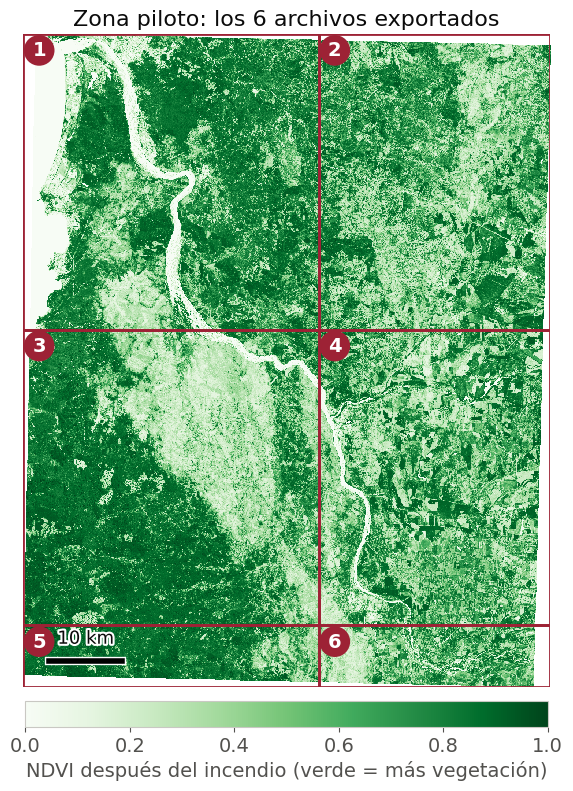
\includegraphics[height=0.84\textheight,keepaspectratio]{ppt_zona_archivos.png}
    \end{column}
  \end{columns}
\end{frame}

\begin{frame}
  \frametitle{Preprocesamiento en Google Earth Engine}
  \small
  \begin{columns}[T]
    \begin{column}{.52\textwidth}
      \textbf{1. Quitar las nubes}
      \begin{itemize}\itemsep0.15em
        \item Solo uso escenas (fotos de una pasada del satélite) con menos de 40\,\% de nubes.
        \item Cada escena trae una capa que dice qué píxeles son nube, sombra, cirro o nieve. Esos píxeles se borran.
        \item Uso 5 bandas (capas de color): azul (B2), rojo (B4), infrarrojo cercano (B8) y dos infrarrojos de onda corta (B11 y B12).
      \end{itemize}
      \vspace{0.3em}
      \textbf{2. Juntar las escenas de cada período}
      \begin{itemize}\itemsep0.15em
        \item Para cada píxel tomo la \textbf{mediana} de todas las escenas del período. Esto se llama compuesto de mediana.
        \item Así desaparecen las nubes que quedaban y \textbf{no queda ningún píxel sin dato}.
      \end{itemize}
    \end{column}
    \begin{column}{.44\textwidth}
      \begin{block}{Tres compuestos}
        \footnotesize
        \begin{tabular}{@{}lll@{}}
          \toprule
          \textbf{Compuesto} & \textbf{Período} & \textbf{Escenas} \\
          \midrule
          Antes del incendio & dic 22 -- ene 23 & 51 \\
          Otoño anterior & mar -- abr 22 & 49 \\
          Después del incendio & mar -- abr 23 & 41 \\
          \bottomrule
        \end{tabular}
      \end{block}
      El otoño anterior sirve para revisar que el modelo no confunda el cambio de estación con un incendio.
    \end{column}
  \end{columns}
\end{frame}

\begin{frame}
  \frametitle{Las tres fechas: la estación cambia poco, el incendio mucho}
  \small
  \begin{center}
    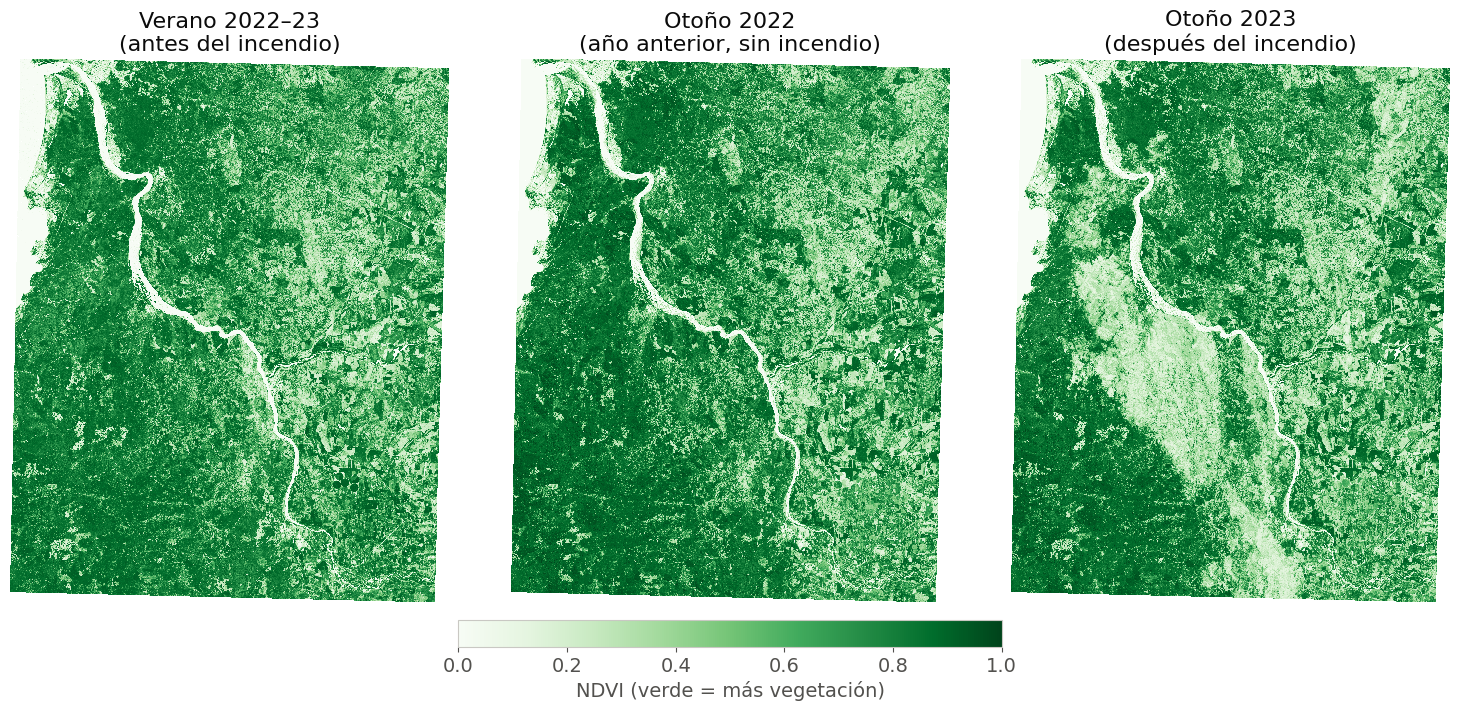
\includegraphics[width=\linewidth,height=0.68\textheight,keepaspectratio]{ppt_estacion.png}
  \end{center}
  \vspace{-0.6em}
  Las dos primeras imágenes no tienen incendio y se parecen mucho, aunque sean de estaciones distintas. En la tercera aparece la \textbf{cicatriz del incendio} en verde claro. Por eso el modelo debería marcar el fuego, no el cambio de estación.
\end{frame}

\begin{frame}
  \frametitle{Cuatro canales: lo que ve el modelo}
  \small
  \begin{columns}[c]
    \begin{column}{.5\textwidth}
      \centering
      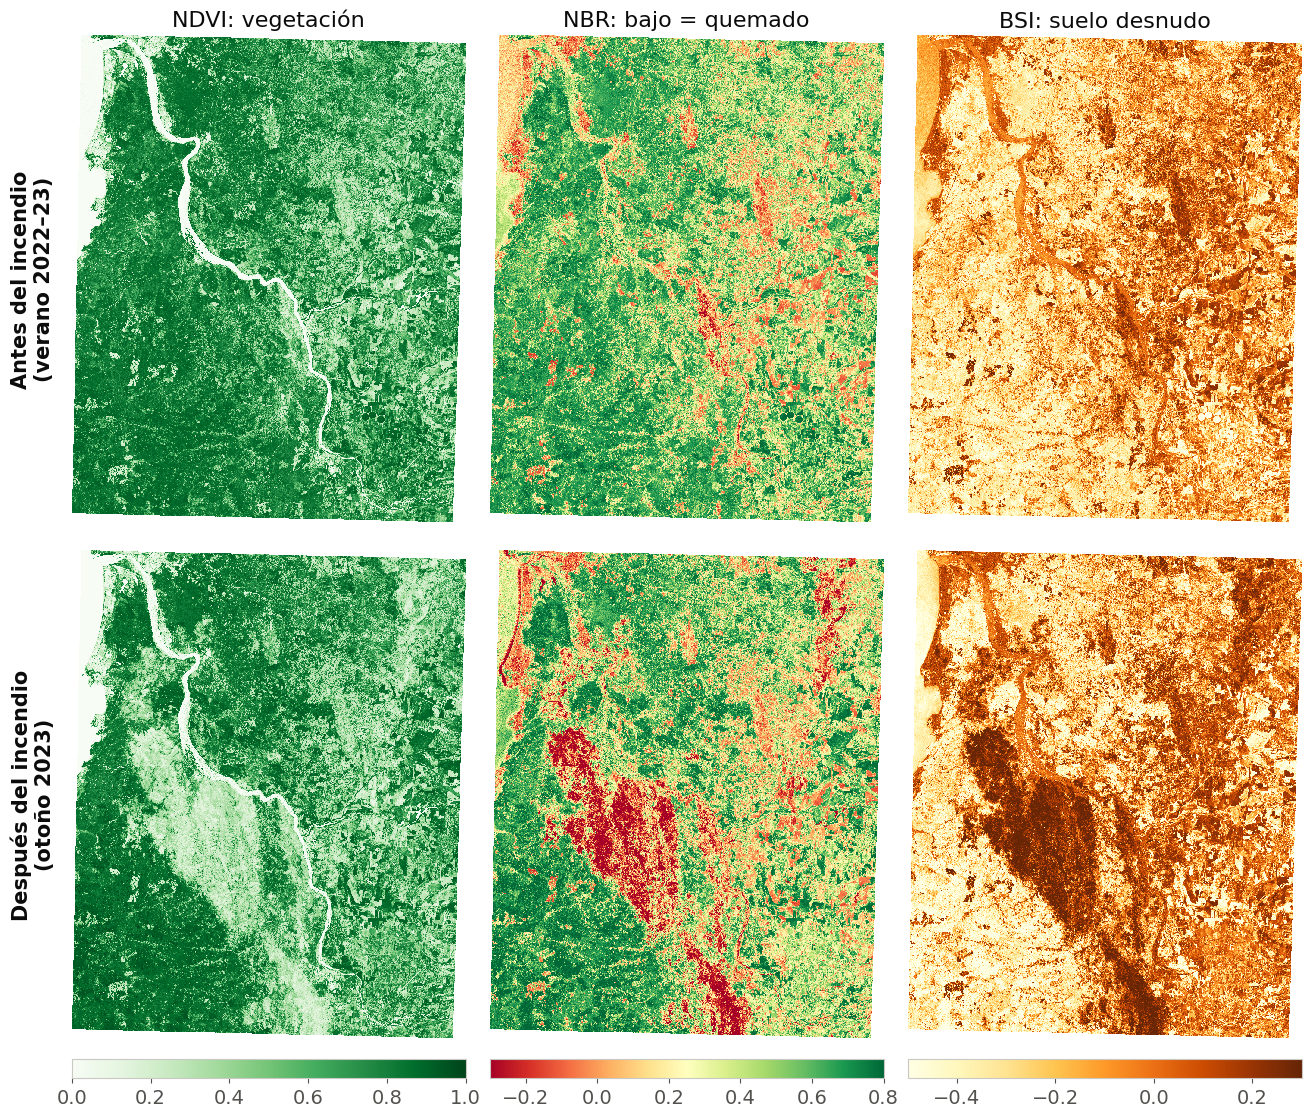
\includegraphics[width=\linewidth,height=0.86\textheight,keepaspectratio]{ppt_antes_despues.png}
    \end{column}
    \begin{column}{.48\textwidth}
      \begin{block}{Qué mide cada canal}
        \begin{itemize}\itemsep0.25em
          \item \textbf{NDVI:} cuánta vegetación verde hay. Después del incendio \textbf{baja} (se pone claro).
          \item \textbf{NBR:} alto = sano, bajo = quemado. En la cicatriz se pone \textbf{rojo}.
          \item \textbf{BSI:} cuánto suelo desnudo hay. En la cicatriz \textbf{sube} (café oscuro).
          \item \textbf{Pendiente:} qué tan inclinado es el terreno. Sale de un modelo de elevación y no cambia con el fuego.
        \end{itemize}
      \end{block}
      \vspace{0.2em}
      {\footnotesize \textbf{Cómo se calculan:} NDVI = (B8 $-$ B4) / (B8 + B4); NBR = (B8 $-$ B12) / (B8 + B12); el BSI combina B2, B4, B8 y B11.}
    \end{column}
  \end{columns}
\end{frame}

\begin{frame}
  \frametitle{Pendiente, máscara y etiquetas de quemado}
  \small
  \begin{center}
    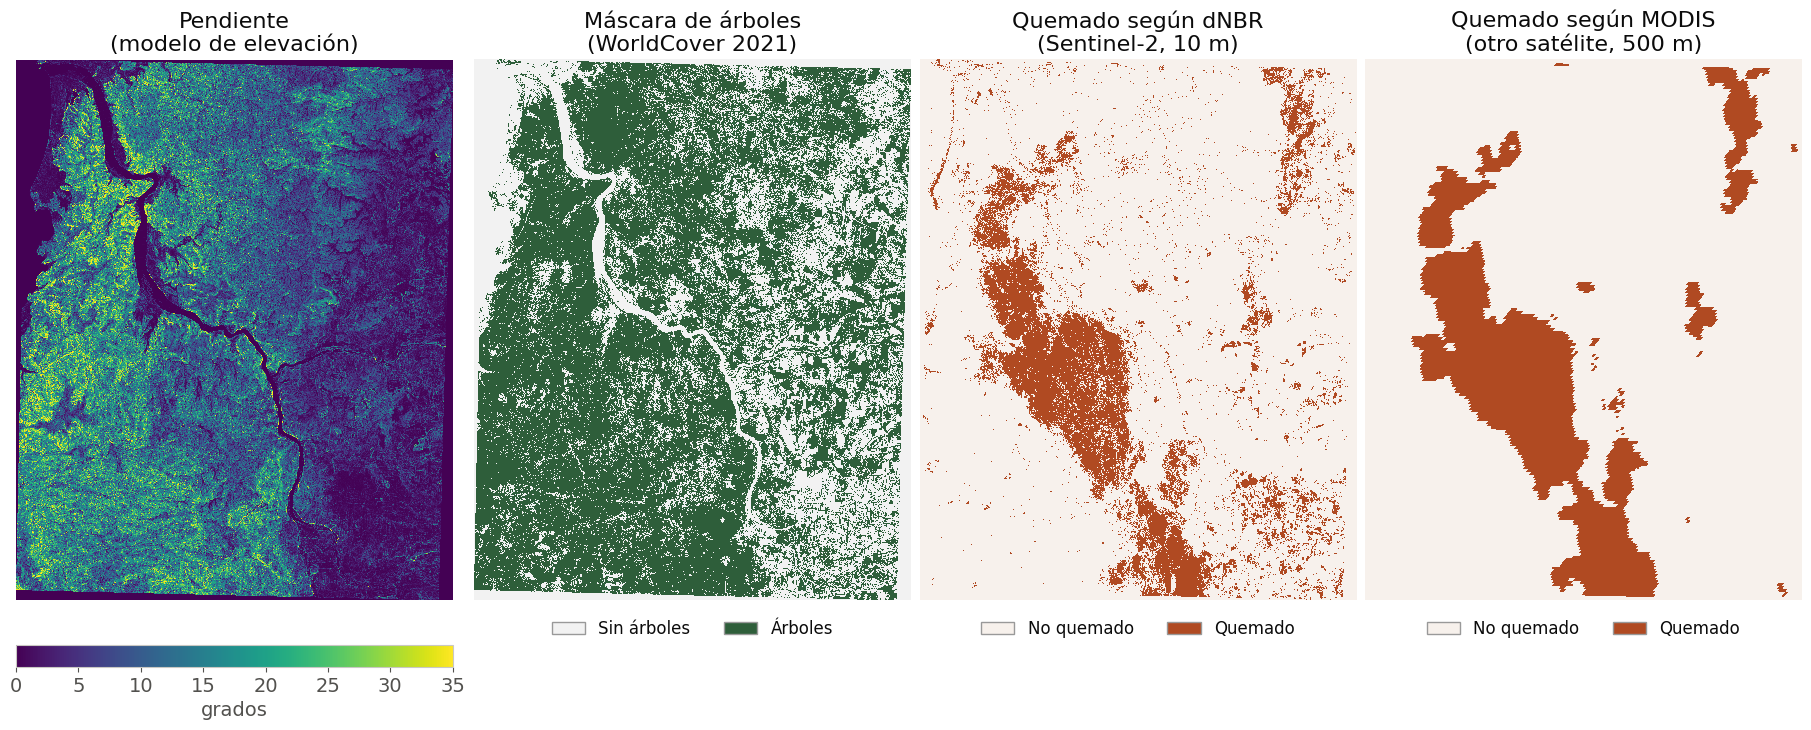
\includegraphics[width=\linewidth,height=0.55\textheight,keepaspectratio]{ppt_pendiente_mascara_etiquetas.png}
  \end{center}
  \vspace{-0.6em}
  \begin{columns}[T]
    \begin{column}{.48\textwidth}
      \begin{itemize}\itemsep0.15em
        \item \textbf{Máscara:} me quedo solo con zonas de árboles (WorldCover 2021). Es provisoria: todavía no separa el pino de otros árboles.
      \end{itemize}
    \end{column}
    \begin{column}{.48\textwidth}
      \begin{itemize}\itemsep0.15em
        \item \textbf{Etiquetas:} quemado si el NBR bajó 0,25 o más (dNBR), y MODIS como segunda opinión. Coinciden bastante (IoU de 0,45 a 0,77).
        \item Las etiquetas \textbf{no se usan para entrenar}, solo para evaluar.
      \end{itemize}
    \end{column}
  \end{columns}
\end{frame}

\begin{frame}
  \frametitle{Construcción de parches y división espacial}
  \small
  \begin{columns}[T]
    \begin{column}{.52\textwidth}
      \begin{itemize}\itemsep0.25em
        \item Corto la zona en parches de \textbf{64 $\times$ 64 píxeles} (640 $\times$ 640 m) y me quedo con los que tienen al menos 80\,\% de árboles: \textbf{6.814 lugares}.
        \item Según cuánto se quemó, cada parche es \textbf{sano} (2\,\% o menos), \textbf{quemado} (50\,\% o más) o \textbf{intermedio} (entre medio).
        \item Separo entrenamiento, validación y test por \textbf{bloques de unos 5 km} (70/15/15), no al azar. Dos parches vecinos se parecen mucho: si uno queda en entrenamiento y el otro en test, el resultado saldría inflado.
        \item Solo en entrenamiento tomo además parches corridos medio parche, para tener más ejemplos.
      \end{itemize}
    \end{column}
    \begin{column}{.44\textwidth}
      \begin{center}
        \footnotesize
        \begin{tabular}{@{}lrrr@{}}
          \toprule
          \textbf{Bloques} & \textbf{Sanos} & \textbf{Quemados} & \textbf{Intermedios} \\
          \midrule
          Entrenamiento & 2.896 & 946 & 818 \\
          Validación & 669 & 172 & 199 \\
          Test & 564 & 312 & 238 \\
          \midrule
          Total & 4.129 & 1.430 & 1.255 \\
          \bottomrule
        \end{tabular}
      \end{center}
      \vspace{0.4em}
      Los intermedios son bordes del incendio. No los uso en el test porque no se sabe bien si contarlos como sanos o como quemados.
    \end{column}
  \end{columns}
\end{frame}

\begin{frame}
  \frametitle{Dataset final y DataLoader}
  \small
  \begin{columns}[T]
    \begin{column}{.45\textwidth}
      \begin{itemize}\itemsep0.15em
        \item En total hay \textbf{29.656 muestras}: los lugares se repiten en las tres fechas, y en entrenamiento se suman los parches corridos.
        \item Cada muestra tiene 4 capas de 64 $\times$ 64 (en total pesan 0,97 GB).
        \item Normalizo cada canal con la media y la desviación del entrenamiento, para que los cuatro queden en escalas parecidas.
        \item Para tener más variedad, volteo los parches al azar.
        \item Un DataLoader de PyTorch entrega los datos al modelo en lotes de 64.
      \end{itemize}
    \end{column}
    \begin{column}{.52\textwidth}
      \begin{center}
        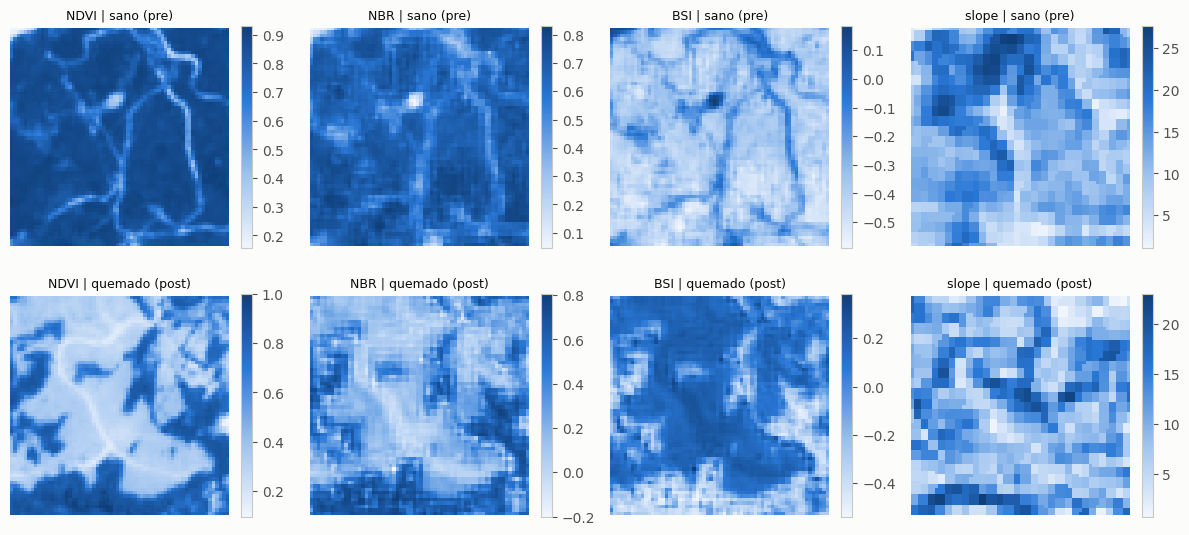
\includegraphics[width=\linewidth,height=0.36\textheight,keepaspectratio]{02_parches_ejemplo.png}
      \end{center}
      \vspace{-0.8em}
      {\footnotesize Arriba, un parche sano antes del incendio; abajo, uno quemado después. En el quemado baja la vegetación (NDVI) y sube el suelo desnudo (BSI).}
      \begin{block}{Uso}
        Entreno con \textbf{10.188 parches sanos} de antes del incendio.\\
        Evalúo con \textbf{564 sanos y 312 quemados} que el modelo nunca vio.
      \end{block}
    \end{column}
  \end{columns}
\end{frame}

% --- SECCIÓN 3 ---
\section[Baseline]{Baseline}

\begin{frame}
  \frametitle{Baseline: primer entrenamiento (E1)}
  \small
  \begin{columns}[T]
    \begin{column}{.4\textwidth}
      \begin{block}{Modelo}
        \begin{itemize}\itemsep0.1em
          \item VAE convolucional: el encoder resume cada parche en 64 números (el latente) y el decoder intenta reconstruirlo desde ese resumen.
          \item Pérdida: error de reconstrucción (MSE) + $\beta\cdot$KL, con $\beta = 0{,}5$. La KL mantiene ordenado el latente.
          \item 50 épocas, unos 3 minutos en una RTX 3060.
        \end{itemize}
      \end{block}
      \begin{block}{Resultado}
        AUROC en test: \textbf{0,806}. Es la probabilidad de que un parche quemado tenga más error que uno sano (0,5 = azar; 1 = perfecto).
      \end{block}
    \end{column}
    \begin{column}{.57\textwidth}
      \vspace{1.2em}
      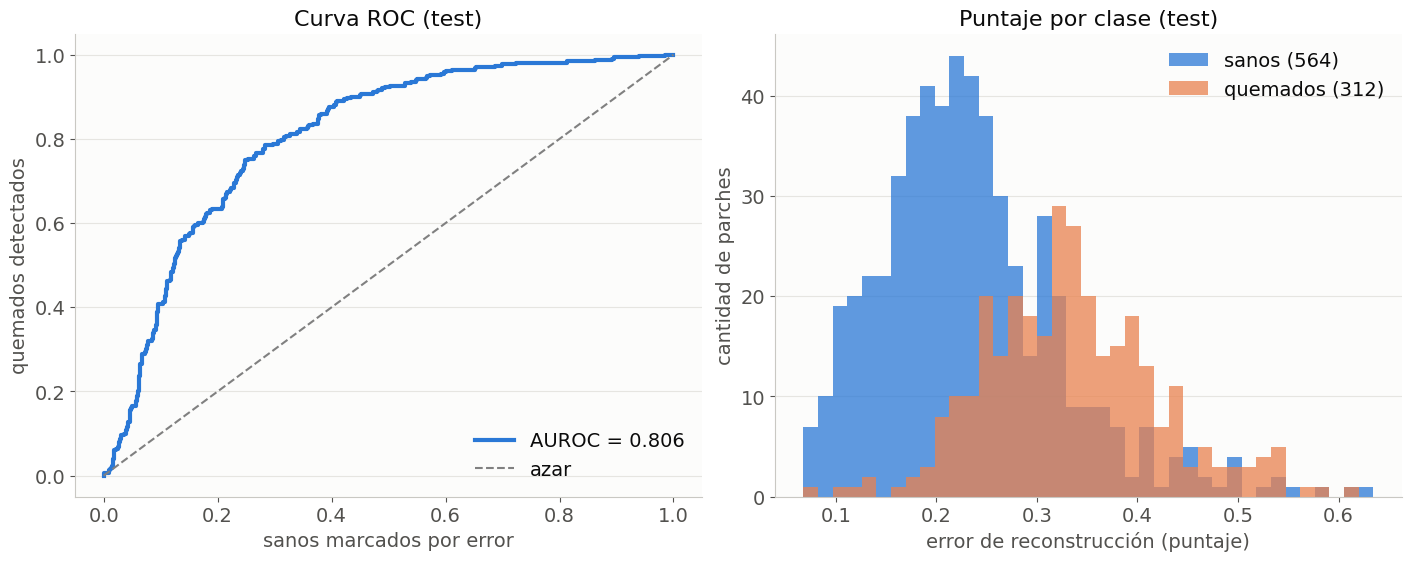
\includegraphics[width=\linewidth,keepaspectratio]{ppt_roc_histograma.png}

      \vspace{0.3em}
      {\footnotesize Izquierda: la curva queda sobre la línea del azar. Derecha: los quemados (naranjo) tienen más error que los sanos (azul), aunque una parte se pisa.}
    \end{column}
  \end{columns}
\end{frame}

% --- SECCIÓN 4 ---
\section[Desafíos]{Desafíos técnicos}

\begin{frame}
  \frametitle{Desafíos técnicos}
  \small
  \begin{block}{Lo que probé (14 entrenamientos, E1 a E7)}
    \begin{itemize}\itemsep0.15em
      \item \textbf{Colapso posterior} (que el modelo ignore el latente): no ocurrió. Las 64 dimensiones del latente cambian según el parche (E1--E3).
      \item \textbf{Peso de la KL ($\beta$):} probé valores de 0 a 4. El mejor fue $\beta = 0{,}1$, con AUROC 0,834 (E3). Subir $\beta$ de a poco (warm-up) ayudó poco (E2).
      \item \textbf{Sobreajuste:} no hay. El error en entrenamiento y en validación es casi igual (E4).
      \item \textbf{¿Detecta el fuego o la estación?} Entrenando con otoño el resultado se mantiene (E5), con la etiqueta de MODIS también (E6), y con 3 semillas distintas da lo mismo (E7).
    \end{itemize}
  \end{block}
  \begin{alertblock}{Desafío abierto: estabilidad}
    La pérdida baja y se estabiliza, pero el AUROC sube y baja entre 0,83 y 0,97 de una época a otra. Pasa porque, al reconstruir cada vez mejor, el modelo también reconstruye mejor lo quemado.\\[0.3em]
    \textbf{Hoy:} elijo el modelo con el error de validación, que sí es estable.
    \textbf{Próximo (E8):} promediar los pesos, bajar la tasa de aprendizaje y usar un latente más chico.
  \end{alertblock}
\end{frame}

% --- SECCIÓN 5 ---
\section[Cierre]{Próximos pasos}

\begin{frame}
  \frametitle{Próximos pasos}
  \begin{itemize}\itemsep0.5em
    \item \textbf{Estabilizar la detección} con el experimento E8.
    \item \textbf{Máscara solo de pino:} usar el catastro de CONAF. Necesito una versión anterior al incendio, para no perder las plantaciones quemadas.
    \item \textbf{Distinguir la causa:} saber si el daño viene de un incendio o de una tala rasa.
    \item \textbf{Métrica generativa:} adaptar el FID, que está pensado para fotos, a imágenes con índices.
  \end{itemize}
  \vspace{1.5em}
  \centering
  \Large ¿Preguntas?
\end{frame}

\end{document}
